%\documentclass[varwidth]{standalone}
\documentclass[
  10pt,
  varwidth,
  border={0pt 0pt 92.5pt 0pt}
]{standalone}

% Standard package includes
\usepackage{times}
\usepackage{latexsym}
\usepackage{booktabs}
\usepackage{hyperref}

% For proper rendering and hyphenation of words containing Latin characters (including in bib files)
\usepackage[T1]{fontenc}
% For Vietnamese characters
% \usepackage[T5]{fontenc}
% See https://www.latex-project.org/help/documentation/encguide.pdf for other character sets

% This assumes your files are encoded as UTF8
\usepackage[utf8]{inputenc}

% This is not strictly necessary, and may be commented out,
% but it will improve the layout of the manuscript,
% and will typically save some space.
\usepackage{microtype}

% This is also not strictly necessary, and may be commented out.
% However, it will improve the aesthetics of text in
% the typewriter font.
\usepackage{inconsolata}

%Including images in your LaTeX document requires adding
%additional package(s)
\usepackage{graphicx}
\usepackage[hyperfirst=false, nonumberlist, nostyles, nogroupskip]{glossaries}

\usepackage{fontawesome5}
\usepackage{pgfplots}
\pgfplotsset{compat=1.18}


\usepackage{tikz}
\usetikzlibrary{shapes.geometric, arrows, positioning, calc, arrows.meta, backgrounds, fit}
\usepackage{booktabs}  % For table rules
%\usepackage[table,xcdraw]{xcolor}    % For coloring
\usepackage{siunitx}   % For number formatting and alignment
\usepackage{tcolorbox} % For rounded corner colored boxes

\usepackage{mathtools}
\usepackage{amssymb}
\usepackage[normalem]{ulem}  % Paket für durchgestrichenen Text
\usepackage{marginnote}
\renewcommand{\marginpar}{\marginnote}
\usepackage{colortbl}
\newcommand{\gradiend}{\textsc{Gradiend}}


\makeatletter
\renewcommand\tiny{\@setfontsize\tiny{5.4pt}{6.2pt}}
\makeatother


\begin{document}

\begin{tikzpicture}[
  font=\sffamily,
  W/.store in=\W, W=2.8cm,
  H/.store in=\H, H=3.4cm,
  gap/.store in=\gap, gap=7mm,
  vgap/.store in=\vgap, vgap=3mm,
  pad/.store in=\pad, pad=2.2mm,
  % --- boxes ---
  box/.style={
    draw=black!20, rounded corners=2mm, fill=white,
    inner sep=\pad, text width=\W, align=left
  },
  topbox/.style={box, minimum height=\H},
  rightbox/.style={box},
  % --- typography ---
  boxtitle/.style={font=\bfseries\footnotesize, text=black!90},
  tiny/.style={font=\tiny, text=black!70},
  % --- API pill ---
  apipill/.style={
    draw=black!18, rounded corners=1.4mm, fill=black!3,
    inner sep=1.2mm, font=\ttfamily\tiny, text=black!70
  },
  % --- visual slot ---
  slot/.style={
    draw=black!15, rounded corners=1.6mm, fill=black!2,
    inner sep=1.8mm, align=center
  },
  % --- process arrows (block/process look) ---
  proc/.style={
    -{Triangle[length=9pt,width=12pt]},
    line width=5.2pt, draw=black!55
  }
]

% =========================
% ACCENT COLORS (one per box)
% =========================
\colorlet{cData}{blue!70!black}
\colorlet{cTrain}{violet!70!black}
\colorlet{cIntra}{green!55!black}
\colorlet{cRewrite}{orange!80!black}
\colorlet{cInter}{red!70!black}

% card border + subtle tint (ONLY color; no geometry)
\tikzset{
  boxData/.style   ={draw=cData!55,   fill=cData!6},
  boxTrain/.style  ={draw=cTrain!55,  fill=cTrain!6},
  boxIntra/.style  ={draw=cIntra!55,  fill=cIntra!6},
  boxRewrite/.style={draw=cRewrite!55,fill=cRewrite!6},
  boxInter/.style  ={draw=cInter!55,  fill=cInter!6},
  % icon coloring helper (use: icon=cData, etc.)
  icon/.style args={#1}{text=#1!85},
  % highlight helper for one element per box
  hi/.style args={#1}{fill=#1!28, draw=#1!70}
}


% global node diameter
\newcommand{\nnDiam}{1mm} 


% right boxes heights so that: H = Hright + vgap + Hright
\pgfmathsetlengthmacro{\Hright}{(\H-\vgap)/2}

% =========================
% BOX LAYOUT
% =========================
\node[topbox, boxData] (B1) {};
\node[topbox, boxTrain, right=\gap of B1] (B2) {};
\node[topbox, boxIntra, right=\gap of B2] (B3) {};

% Right column: north-aligned + south-aligned to the top row
\node[rightbox, boxRewrite, minimum height=\Hright, anchor=north west]
  (B4a) at ([xshift=\gap]B3.north east) {};
\node[rightbox, boxInter, minimum height=\Hright, anchor=south west]
  (B4b) at ([xshift=\gap]B3.south east) {};

% =========================
% PROCESS ARROWS (horizontal + parallel)
% =========================
\draw[proc] (B1.east) -- (B2.west);
\draw[proc] (B2.east) -- (B3.west);

\coordinate (S4a) at (B3.east|-B4a.west);
\coordinate (S4b) at (B3.east|-B4b.west);
\draw[proc] (S4a) -- (B4a.west);
\draw[proc] (S4b) -- (B4b.west);

% =========================
% HELPERS: title + api pill + one or two visual slots
% (No \dimexpr multiplication; use "2\pad" not "2*\pad")
% =========================
\tikzset{
  boxtitle/.style={font=\bfseries\footnotesize, text=black!90},
  bodytiny/.style={font=\tiny, text=black!80, align=left},
  apipill/.style={
    draw=black!18, rounded corners=1.4mm, fill=black!3,
    inner sep=0.7mm, font=\ttfamily\tiny, text=black!70
  },
  inset/.style={
    draw=black!15, rounded corners=1.6mm, fill=black!2,
    inner sep=2.0mm, align=left
  },
  chevron/.style={-Latex, line width=0.9pt, draw=black!55}
}

% --- Helper: title + api anchored to padded corners (works best if your box uses inner xsep/ysep) ---
\newcommand{\PlaceTitleApi}[3]{%
  % Title (unchanged)
  \node[anchor=north west, boxtitle, 
    text width=2.6cm,]
    at (#1.north west) {\scriptsize #2};

  % API pill slightly outside bottom-right
  \node[
    anchor=south east,
    apipill,
  ] at ([xshift=2.5mm,yshift=-2.5mm]#1.south east) {\tiny #3};
}


\newcommand{\DataExample}[1]{%
  % Inner example box (positioned under title)
  \node[inset, anchor=north west, text width=\W-8mm] (ex#1) at ([yshift=-7mm]#1.north west) {%
    \bodytiny
    \textbf{Text:} Mary said that \texttt{[MASK]} arrived.\par\vspace{0.8mm}
    \textbf{Factual:} \texttt{[MASK]} $=$ ``she''\par
    \textbf{Counterfactual:} \texttt{[MASK]} $=$ ``he''
  };

  % Arrow / explanation line under the inner box
  \node[bodytiny, anchor=north west] (grad#1) at ([yshift=-2mm]ex#1.south west) {%
    $\rightarrow$ MLM/CLM gradients $\nabla_\theta$ \;\; $\rightarrow$ feature direction $\Delta\theta$
  };
}

% =========================
% CONTENT (minimal text, visual placeholders)
% =========================

% Data: example text (later: real mini rendered example or a tiny PDF/PNG)
\PlaceTitleApi{B1}{Feature Selection and Data Generation}{TextPredictionDataCreator()}
\node[
  anchor=north east,
  text=teal!80!black,
  scale=0.95, icon=cData,
] at ([xshift=-0.5mm,yshift=-0.0mm]B1.north east)
{\faIcon{file-alt}};
% =========================
% DATA CONTENT (modern card style)
% =========================

% Title
\node[
  anchor=north west,
  font=\tiny,
  text=black!90,
  text width=3.05cm,
  text=black!65,
] at ([yshift=-6.7mm, xshift=0mm]B1.north west)
%{Feature described by two target classes (e.g., gender: female/male)};
%{Two target classes specify \\the feature axis (e.g., \emph{female} vs.\ \emph{male} for feature \emph{gender})};
%{Two target classes specify \\the feature axis (e.g., \emph{female} vs.\ \emph{male} for feature \emph{grammatical person})};
{Two classes define the feature axis (e.g., 3rd-person singular vs.\ plural (\emph{3SG} vs.\ \emph{3PL}) for \emph{gram.\ number})};



% API pill
% Inner example card (centered with clean margins)
\iffalse
\node[
  draw=black!15,
  rounded corners=1.6mm,
  fill=black!1,
  inner sep=1mm,
  align=left,
  text=black!80,
  font=\tiny,
  text width=\W-0mm,
  anchor=north west
] (dataex) at ([yshift=-13mm, xshift=1mm]B1.north west)
{
\textbf{Text}\, 
%Mary said that \texttt{\textcolor{cData}{\textbf{[MASK]}}} arrived.\par\vspace{1mm}
The nurse Mary said that \texttt{\textcolor{cData}{\textbf{[MASK]}}} was exhausted.\par\vspace{1mm}

\textbf{Factual}\, \texttt{\textcolor{cData}{\textbf{[MASK]}}} = ``she''\par\vspace{1mm}
\textbf{Counterfactual}\, \texttt{\textcolor{cData}{\textbf{[MASK]}}} = ``he''
};
\fi
\node[
  draw=black!15,
  rounded corners=1.6mm,
  fill=black!1,
  inner sep=0.8mm,
  align=left,
  text=black!80,
  font=\fontsize{5.7pt}{6.1pt}\selectfont,,
  text width=\W-0mm,
  anchor=north west
] (dataex) at ([yshift=-15.5mm, xshift=1.3mm]B1.north west)
{
\textbf{Text}\, 
%Mary said that \texttt{\textcolor{cData}{\textbf{[MASK]}}} arrived.\par\vspace{1mm}
The nurse Mary said that \texttt{\textcolor{cData}{\textbf{[MASK]}}} was exhausted.\par\vspace{1mm}

\textbf{Factual}\, \texttt{\textcolor{cData}{\textbf{[MASK]}}} = ``she''\par\vspace{1mm}
\textbf{Counterfactual}\, \texttt{\textcolor{cData}{\textbf{[MASK]}}} = ``they''
};

% Gradient explanation line (subtle)
\node[
  anchor=north west,
  font=\tiny,
  text=black!65,
   text width=3.cm,
  align=left
] at ([yshift=-27.0mm]B1.north west)
{The MLM/CLM gradients are used as model inputs and outputs};



% GRADIEND: network diagram (later: \includegraphics)
\PlaceTitleApi{B2}{\gradiend\ Training}{Trainer.train()}
\node[
  anchor=north east,
  text=teal!80!black,
  scale=0.95,
  icon=cTrain
] at ([xshift=-0.5mm,yshift=-0.0mm]B2.north east)
{\faIcon{cogs}};
%{\faIcon{project-diagram}};
%{\faIcon{chart-line}};

\begin{scope}[shift={([yshift=-1.9mm, xshift=0mm]B2.center)}, x=1mm,y=1mm]

  % x positions (simple)
  \def\xI{-8}
  \def\xF{0}
  \def\xO{8}

  % styles (match your look)
  \tikzset{
    nnode/.style={circle,draw=black!35,fill=white,minimum size=2.5mm,inner sep=0pt,line width=0.35pt},
    nhot/.style ={circle,draw=black!35,fill=cTrain!55,minimum size=2.5mm,inner sep=0pt,line width=0.35pt},
    nedge/.style={draw=black!25,line width=0.50pt},
    featArrow/.style={-Latex, draw=black!55, line width=0.45pt},
    featLabel/.style={font=\tiny, text=black!70}
  }

  % 8 y positions (top to bottom)
  \def\yone{10.5}
  \def\ytwo{7.5}
  \def\ythree{4.5}
  \def\yfour{1.5}
  \def\yfive{-1.5}
  \def\ysix{-4.5}

  % INPUT nodes I1..I8
  \node[nnode] (I1) at (\xI,\yone) {};
  \node[nnode] (I2) at (\xI,\ytwo) {};
  \node[nnode] (I3) at (\xI,\ythree) {};
  \node[nnode] (I4) at (\xI,\yfour) {};
  \node[nnode] (I5) at (\xI,\yfive) {};
  \node[nnode] (I6) at (\xI,\ysix) {};

  % FEATURE latent node
  \node[nhot] (F) at (\xF,3) {};

  % OUTPUT nodes O1..O8
  \node[nnode] (O1) at (\xO,\yone) {};
  \node[nnode] (O2) at (\xO,\ytwo) {};
  \node[nnode] (O3) at (\xO,\ythree) {};
  \node[nnode] (O4) at (\xO,\yfour) {};
  \node[nnode] (O5) at (\xO,\yfive) {};
  \node[nnode] (O6) at (\xO,\ysix) {};

  % Connections: inputs -> feature
  \foreach \i in {1,2,3,4,5,6} {
    \draw[nedge] (I\i) -- (F);
  }

  % Connections: feature -> outputs
  \foreach \j in {1,2,3,4,5,6} {
    \draw[nedge] (F) -- (O\j);
  }

  % Label "feature" with arrow to latent node
  \node[featLabel] (flab) at ([xshift=0mm,yshift=-5.2mm]F.south) {feature $h$};
  \draw[featArrow] (flab.north) -- (F);
\node[featLabel] (enc) at ([xshift=0mm,yshift=1.4mm]I1.north) {Encoder};
  \node[featLabel] (dec) at ([xshift=0mm,yshift=1.4mm]O1.north) {Decoder};

% --- Encoder/Decoder background boxes + captions ---
\begin{pgfonlayer}{background}
  % left (encoder) box
  \node[
    fit=(I1)(I6),
    inner sep=1.2mm,
    rounded corners=0.8mm,
    fill=black!3,
    draw=black!15,
    line width=0.25pt
  ] (encBox) {};

  % right (decoder) box
  \node[
    fit=(O1)(O6),
    inner sep=1.2mm,
    rounded corners=0.8mm,
    fill=black!3,
    draw=black!15,
    line width=0.25pt
  ] (decBox) {};
\end{pgfonlayer}

% captions under boxes
\node[featLabel, align=center, text=black!65, text width=1.5cm]
  at ([yshift=-3mm, xshift=-0.0mm]encBox.south) {Encoding a scalar feature value};

\node[featLabel, align=center, text=black!65,  text width=1.5cm]
  at ([yshift=-3mm, xshift=-0.0mm]decBox.south) { Decoding model feature update direction};



% 
%
  
\end{scope}




% Intra Eval: encoder + decoder plots (two slots)
\PlaceTitleApi{B3}{Intra-Model Evaluation}{Trainer.evaluate()}
\node[
  anchor=north east,
  text=teal!80!black,
  scale=0.95,
  icon=cIntra
] at ([xshift=-0.5mm,yshift=-0.0mm]B3.north east)
{\faIcon{chart-bar}};


\node[
  anchor=north west,
  font=\tiny,
  text width=3.1cm,
  text=black!65,
] at ([yshift=-4mm, xshift=0mm]B3.north west)
{Encoder analysis: are feature classes separated?};


\begin{scope}[shift={([yshift=0mm, xshift=-8mm]B3.center)}]

  \colorlet{vPlus}{cIntra!75}
  \colorlet{vMinus}{cIntra!50}
  \colorlet{vZero}{cIntra!28}

  \begin{axis}[
    width=3.2cm, height=2.2cm,
    xmin=0.60, xmax=1.6,     % <-- tighter + gives left margin
    ymin=-1.05, ymax=1.05,
    axis x line*=bottom,
    axis y line*=left,
    xtick=\empty,
    ytick={-1,0,1},
    yticklabels={-1,0,+1},
    ticklabel style={font=\fontsize{4.8pt}{5.4pt}\selectfont, text=black!65},
    axis line style={draw=black!20, line width=0.3pt},
    tick style={draw=black!20, line width=0.3pt},
    clip=false,
    ylabel={$h$},
    enlargelimits=0.05,
ylabel style={
  font=\fontsize{4.5pt}{5pt}\selectfont,
  text=black!70,
  yshift=-1.5mm,
},
  ]

  % split violin center line
  \addplot[draw=black!25, line width=0.25pt] coordinates {(1,-1.0) (1,1.0)};

  % LEFT HALF (+1) — peak pushed closer to +1 (bulge very near top)
  \path[draw=black!25, line width=0.25pt, fill=vPlus]
    (axis cs:1,0.50)
    .. controls (axis cs:1-0.01,0.50) and (axis cs:1-0.14,0.72) ..
    (axis cs:1-0.22,0.82)
    .. controls (axis cs:1-0.36,0.93) and (axis cs:1-0.30,0.995) ..
    (axis cs:1,1.00)
    -- (axis cs:1,0.50) -- cycle;

  % RIGHT HALF (-1) — peak pushed closer to -1 (bulge very near bottom)
  \path[draw=black!25, line width=0.25pt, fill=vMinus]
    (axis cs:1,-1.00)
    .. controls (axis cs:1+0.01,-1.00) and (axis cs:1+0.18,-0.985) ..
    (axis cs:1+0.32,-0.93)
    .. controls (axis cs:1+0.36,-0.88) and (axis cs:1+0.22,-0.68) ..
    (axis cs:1,-0.50)
    -- (axis cs:1,-1.00) -- cycle;

  % 0 violin at x=1.62 (slightly closer, to reduce empty space)
  \addplot[draw=black!25, line width=0.25pt] coordinates {(1.62,-0.5) (1.62,0.5)};

  % left half (0)
  \path[draw=black!25, line width=0.25pt, fill=vZero]
    (axis cs:1.62,-0.50)
    .. controls (axis cs:1.62-0.02,-0.50) and (axis cs:1.62-0.22,-0.25) ..
    (axis cs:1.62-0.28,0.00)
    .. controls (axis cs:1.62-0.22,0.25) and (axis cs:1.62-0.02,0.50) ..
    (axis cs:1.62,0.50)
    -- (axis cs:1.62,-0.50) -- cycle;

  \end{axis}


% --- LABELS ---

% Feature class 1 (oben links, +1 Hälfte)
\draw[black!40, line width=0.25pt]
  (rel axis cs:0.33,0.92) -- ++(2mm,0);
\node[anchor=west, font=\fontsize{4.2pt}{5pt}\selectfont, text=black!75]
  at ([xshift=1mm]rel axis cs:0.33,0.92)
  {feature class $A$};

% Feature class 2 (unten rechts, -1 Hälfte)
\draw[black!40, line width=0.25pt]
  (rel axis cs:0.6,0.08) -- ++(2mm,0);
\node[anchor=west, font=\fontsize{4.2pt}{5pt}\selectfont, text=black!75]
  at ([xshift=1mm]rel axis cs:0.6,0.08)
  {feature class $B$};

% Neutral inputs (rechtes Violin)
\draw[black!40, line width=0.25pt]
  (rel axis cs:0.96,0.55) -- ++(2mm,0);
\node[anchor=west, font=\fontsize{4.2pt}{5pt}\selectfont, text=black!75]
  at ([xshift=1mm]rel axis cs:0.96,0.55)
  {neutral};
  
\end{scope}


\node[
  anchor=north west,
  font=\tiny,
  text=black!65,
  text width=3.cm,
] at ([yshift=-18mm, xshift=0mm]B3.north west)
{Decoder analysis: change probabilities of feature tokens};

\begin{scope}[shift={([yshift=-14mm, xshift=-8mm]B3.center)}]

\colorlet{pDark}{cIntra!70}
\colorlet{pLight}{cIntra!30}

\begin{axis}[
  width=3.2cm, height=2.2cm,
  xmode=log,
  xmin=1e-6, xmax=1e-1,
  ymin=0, ymax=1,
  xlabel={learning rate},
  ylabel={$\mathbb{P}$},
  xlabel style={font=\fontsize{4.8pt}{5.3pt}\selectfont, text=black!75, yshift=3.5mm},
  ylabel style={font=\fontsize{4.8pt}{5.3pt}\selectfont, text=black!75, yshift=-1.5mm,},
  ytick={0,0.5,1},
  yticklabels={0,0.5,1},
  ticklabel style={font=\fontsize{4.0pt}{4.6pt}\selectfont, text=black!65},
  axis line style={draw=black!20, line width=0.3pt},
  tick style={draw=black!20, line width=0.3pt},
  clip=false,
  xticklabels=\empty,
  enlargelimits=0.05,
]



% dark: high -> low
\addplot[
  smooth,
  mark=o,
  mark size=0.5pt,
  line width=0.7pt,
  draw=pLight
] coordinates {
  (1.000e-6, 0.95)
  (2.848e-6, 0.94)
  (8.111e-6, 0.92)
  (2.310e-5, 0.88)
  (6.579e-5, 0.80)
  (1.874e-4, 0.65)
  (5.336e-4, 0.50)
  (1.520e-3, 0.35)
  (4.328e-3, 0.20)
  (1.233e-2, 0.12)
  (3.511e-2, 0.07)
  (1.000e-1, 0.05)
};

% light: low -> high
\addplot[
  smooth,
  mark=o,
  mark size=0.5pt,
  line width=0.7pt,
  draw=pDark,
] coordinates {
  (1.000e-6, 0.05)
  (2.848e-6, 0.06)
  (8.111e-6, 0.08)
  (2.310e-5, 0.12)
  (6.579e-5, 0.20)
  (1.874e-4, 0.35)
  (5.336e-4, 0.50)
  (1.520e-3, 0.65)
  (4.328e-3, 0.80)
  (1.233e-2, 0.88)
  (3.511e-2, 0.93)
  (1.000e-1, 0.95)
};

\end{axis}
\end{scope}


\node[
  anchor=north west,
  font=\fontsize{4.5pt}{5.3pt}\selectfont,
  text=black!65,
  text width=3.cm,
] at ([yshift=-23mm, xshift=24mm]B3.north west)
{$\mathbb{P}(A)$};
\node[
  anchor=north west,
  font=\fontsize{4.5pt}{5.3pt}\selectfont,
  text=black!65,
  text width=3.cm,
] at ([yshift=-28.5mm, xshift=24mm]B3.north west)
{$\mathbb{P}(B)$};


% Deployment: rewrite visual
\PlaceTitleApi{B4a}{Model Rewrite}{Trainer.rewrite\_base\_model()}




% --- Connected Neural Network ---
% --- Visual slot container ---
\node[
  anchor=west,
  align=left,
  text width=1.4cm,   % <-- adjust width
  font=\tiny,
  text=black!65,
] (rewriteText)
at ([xshift=0mm, yshift=-1.6mm]B4a.west)
{Modify model behavior
along learned feature direction};


% --- Connected Neural Network (5 layers total) ---
\begin{scope}[shift={([yshift=-1.5mm, xshift=8mm]B4a.center)}, x=1mm,y=1mm]

  % symmetric x positions -> centered around 0
  \def\xI{-6}
  \def\xHone{-3}
  \def\xHtwo{0}
  \def\xHthree{3}
  \def\xO{6}

  \tikzset{
    nnode/.style={circle,draw=black!35,fill=white,minimum size=1.5mm,inner sep=0pt,line width=0.35pt},
    nhot/.style ={circle,draw=black!35,fill=cRewrite!55,minimum size=1.5mm,inner sep=0pt,line width=0.35pt},
    nedge/.style={draw=black!25,line width=0.30pt}
  }

  % y positions
  \def\yA{3} \def\yB{1} \def\yC{-1} \def\yD{-3}

  % INPUT (random highlights)
  \node[nnode] (I1) at (\xI,\yA) {};
  \node[nhot]  (I2) at (\xI,\yB) {};
  \node[nnode] (I3) at (\xI,\yC) {};
  \node[nhot]  (I4) at (\xI,\yD) {};

  % H1
  \node[nnode] (H11) at (\xHone,2) {};
  \node[nhot]  (H12) at (\xHone,0) {};
  \node[nnode] (H13) at (\xHone,-2) {};

  % H2
  \node[nhot]  (H21) at (\xHtwo,2) {};
  \node[nnode] (H22) at (\xHtwo,0) {};
  \node[nnode] (H23) at (\xHtwo,-2) {};

  % H3
  \node[nnode] (H31) at (\xHthree,2) {};
  \node[nnode] (H32) at (\xHthree,0) {};
  \node[nhot]  (H33) at (\xHthree,-2) {};

  % OUTPUT (random highlights)
  \node[nhot] (O1) at (\xO,\yA) {};
  \node[nnode]  (O2) at (\xO,\yB) {};
  \node[nhot] (O3) at (\xO,\yC) {};
  \node[nnode]  (O4) at (\xO,\yD) {};

  % Connections
  \foreach \i in {1,2,3,4}
    \foreach \j in {1,2,3}
      \draw[nedge] (I\i) -- (H1\j);

  \foreach \i in {1,2,3}
    \foreach \j in {1,2,3}
      \draw[nedge] (H1\i) -- (H2\j);

  \foreach \i in {1,2,3}
    \foreach \j in {1,2,3}
      \draw[nedge] (H2\i) -- (H3\j);

  \foreach \i in {1,2,3}
    \foreach \j in {1,2,3,4}
      \draw[nedge] (H3\i) -- (O\j);

\end{scope}

% --- Pen icon overlay (top-right inside slot) ---
\node[
  anchor=north east,
  text=teal!80!black,
  scale=0.95,
  icon=cRewrite
] at ([xshift=-0.5mm,yshift=-0.0mm]B4a.north east)
{\faIcon{pen}};





% Comparison: venn + heatmap (two slots)
\PlaceTitleApi{B4b}{Inter-Model Evaluation}{plot\_topk\_overlap()}
\node[
  anchor=north east,
  text=teal!80!black,
  scale=0.95,
  icon=cInter
] at ([xshift=-0.5mm,yshift=-0.0mm]B4b.north east)
{\faIcon{clone}};
%\faIcon{layer-group}
%\faIcon{clone} th


\node[
  anchor=north,
  align=left,
  text width=2.4cm,   % <-- adjust width
  font=\tiny,
  text=black!65,
] (rewriteText)
at ([xshift=-3mm, yshift=-3mm]B4b.north)
{Compare multiple features};

\begin{scope}[shift={([yshift=-3mm, xshift=-6mm]B4b.center)}, x=1mm,y=1mm]
    % --- tune ---
\def\rA{3}
  \def\rB{3}
  \def\rC{3}

  % Make A and B more similar (strong overlap), C a bit farther away
  \coordinate (A) at (-2,  0.0);
  \coordinate (B) at ( 1.2,  -0.8);
  \coordinate (C) at ( 1.5,  1.5);

  % --- base colors: 3 variants of the same family ---
  \colorlet{cA}{cInter!92!black}  % slightly darker
  \colorlet{cB}{cInter!75!black}  % medium
  \colorlet{cC}{cInter!60!black}  % lighter

  % --- fills: transparency yields overlap "combinations" automatically ---
  \def\op{0.17}

  \fill[cA, fill opacity=\op, draw=none] (A) circle (\rA);
  \fill[cB, fill opacity=\op, draw=none] (B) circle (\rB);
  \fill[cC, fill opacity=\op, draw=none] (C) circle (\rC);

  % outlines
  \draw[draw=cA!80, line width=0.6pt] (A) circle (\rA);
  \draw[draw=cB!80, line width=0.6pt] (B) circle (\rB);
  \draw[draw=cC!80, line width=0.6pt] (C) circle (\rC);

  % optional labels (tiny)
  \node[font=\tiny, text=cA!85] at ($(A)+(-3.9, 0)$) {\fontsize{4.3pt}{5.2pt}\selectfont$A \!\rightleftarrows\! B$};
  \node[font=\tiny, text=cB!85] at ($(B)+( 2, -2)$) {\fontsize{4.3pt}{5.2pt}\selectfont$B\!\leftrightarrows\! C$};
  \node[font=\tiny, text=cC!85] at ($(C)+( 2,1.8)$) {\fontsize{4.3pt}{5.2pt}\selectfont$A\!\leftrightarrows\! C$};
\end{scope}

\begin{scope}[shift={([yshift=-5.5mm, xshift=6mm]B4b.center)}, x=1mm,y=1mm,  scale=0.65]

  \def\n{6}
  \def\cell{1.7}   % unitless (mm via x=1mm)
  \def\gap{0.0}
  \def\lw{0.18}    % pt-ish; used as line width in pt below

  % derived geometry (unitless coords)
  \pgfmathsetmacro{\step}{\cell+\gap}
  \pgfmathsetmacro{\size}{\n*\step}

  % helper: i=1..6 left->right, j=1..6 top->bottom
  \newcommand{\Cell}[3]{%
    \pgfmathsetmacro{\xx}{(#1-1)*\step}
    \pgfmathsetmacro{\yy}{(\n-#2)*\step} % flip y so j=1 is TOP
    \path[draw=black!10, line width=\lw pt, fill=cInter!#3]
      (\xx,\yy) rectangle ++(\cell,\cell);
  }

  % ===== intensities (higher -> darker), symmetric pairs =====
  % A row/col
  \Cell{1}{1}{100}
 % \Cell{2}{1}{68} \Cell{1}{2}{68}
  %\Cell{3}{1}{62} \Cell{1}{3}{62}
  \Cell{4}{1}{24} \Cell{1}{4}{24}
  \Cell{5}{1}{46} \Cell{1}{5}{46}
  \Cell{6}{1}{20} \Cell{1}{6}{20}

% UL 3x3 off-diagonals (randomized but still dark) — keep symmetric
\Cell{2}{1}{44} \Cell{1}{2}{44} % A-B
\Cell{3}{1}{54} \Cell{1}{3}{54} % A-C



  % B row/col
  \Cell{2}{2}{100}
%  \Cell{3}{2}{66} \Cell{2}{3}{66}
  \Cell{3}{2}{65} \Cell{2}{3}{65} % B-C
  \Cell{4}{2}{22} \Cell{2}{4}{22}
  \Cell{5}{2}{26} \Cell{2}{5}{26}
  \Cell{6}{2}{18} \Cell{2}{6}{18}

  % C row/col
  \Cell{3}{3}{100}
  \Cell{4}{3}{21} \Cell{3}{4}{21}
  \Cell{5}{3}{23} \Cell{3}{5}{23}
  \Cell{6}{3}{17} \Cell{3}{6}{17}

  % D row/col
  \Cell{4}{4}{100}
  \Cell{5}{4}{19} \Cell{4}{5}{19}
  \Cell{6}{4}{16} \Cell{4}{6}{16}

  % E row/col (LR block darker)
  \Cell{5}{5}{100}
  \Cell{6}{5}{64} \Cell{5}{6}{64}

  % F
  \Cell{6}{6}{100}

  % outer border (robust numeric coords)
  \draw[draw=black!12, line width=0.25pt] (0,0) rectangle (\size,\size);

  % ===== labels (compute positions first; avoids "No shape named 6*(...)" errors) =====
  \pgfmathsetmacro{\yA}{(5+0.5)*\step}
  \pgfmathsetmacro{\yB}{(4+0.5)*\step}
  \pgfmathsetmacro{\yC}{(3+0.5)*\step}
  \pgfmathsetmacro{\yD}{(2+0.5)*\step}
  \pgfmathsetmacro{\yE}{(1+0.5)*\step}
  \pgfmathsetmacro{\yF}{(0+0.5)*\step}

  \node[anchor=east, text=black!60] at (1.4,\yA) {\scalebox{0.3}{$A$}};
  \node[anchor=east, text=black!60] at (1.4,\yB) {\scalebox{0.3}{$B$}};
  \node[anchor=east, text=black!60] at (1.4,\yC) {\scalebox{0.3}{$C$}};
  \node[anchor=east, text=black!60] at (1.4,\yD) {\scalebox{0.3}{$D$}};
  \node[anchor=east, text=black!60] at (1.4,\yE) {\scalebox{0.3}{$E$}};
  \node[anchor=east, text=black!60] at (1.4,\yF) {\scalebox{0.3}{$F$}};

  \pgfmathsetmacro{\xA}{(0+0.5)*\step}
  \pgfmathsetmacro{\xB}{(1+0.5)*\step}
  \pgfmathsetmacro{\xC}{(2+0.5)*\step}
  \pgfmathsetmacro{\xD}{(3+0.5)*\step}
  \pgfmathsetmacro{\xE}{(4+0.5)*\step}
  \pgfmathsetmacro{\xF}{(5+0.5)*\step}

  \node[anchor=north, text=black!60] at (\xA,1.5) {\scalebox{0.3}{$A$}};
  \node[anchor=north, text=black!60] at (\xB,1.5) {\scalebox{0.3}{$B$}};
  \node[anchor=north, text=black!60] at (\xC,1.5) {\scalebox{0.3}{$C$}};
  \node[anchor=north, text=black!60] at (\xD,1.5) {\scalebox{0.3}{$D$}};
  \node[anchor=north, text=black!60] at (\xE,1.5) {\scalebox{0.3}{$E$}};
  \node[anchor=north, text=black!60] at (\xF,1.5) {\scalebox{0.3}{$F$}};
\end{scope}


\end{tikzpicture}


\end{document}
